% This file was created by matplotlib2tikz v0.6.14.
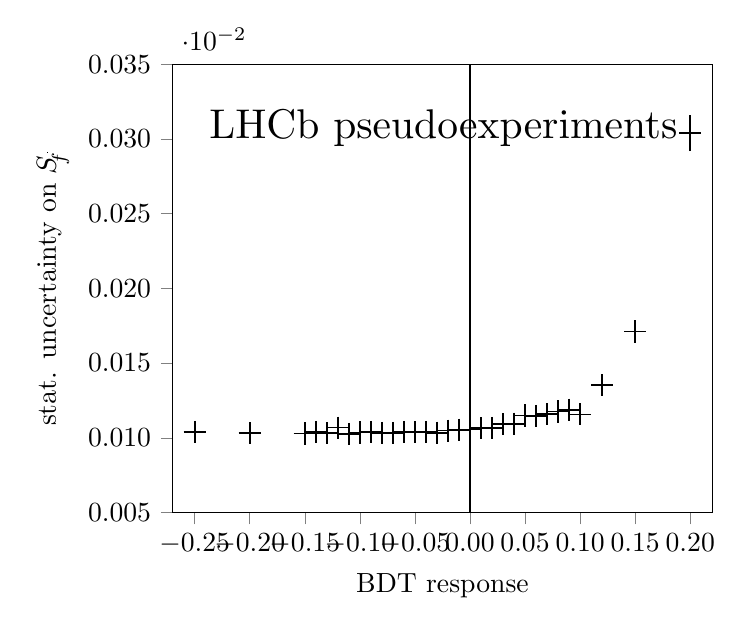
\begin{tikzpicture}

\begin{axis}[
xlabel={BDT response},
ylabel={stat. uncertainty on $S_{\kern 1.7pt\overline{\kern -4.7pt f\kern 0.2pt}}$},
xmin=-0.27, xmax=0.22,
ymin=0.005, ymax=0.035,
xtick={-0.3,-0.25,-0.2,-0.15,-0.1,-0.05,5.55111512312578e-17,0.05,0.1,0.15,0.2,0.25},
xticklabels={,$-0.25$,$-0.20$,$-0.15$,$-0.10$,$-0.05$,$0.00$,$0.05$,$0.10$,$0.15$,$0.20$,},
ytick={0,0.005,0.01,0.015,0.02,0.025,0.03,0.035,0.04},
yticklabels={,$0.005$,$0.010$,$0.015$,$0.020$,$0.025$,$0.030$,$0.035$,},
tick align=outside,
tick pos=left,
x grid style={white!69.019607843137251!black},
y grid style={white!69.019607843137251!black}
]
\path [draw=black, semithick] (axis cs:-0.25,0.0103764436508139)
--(axis cs:-0.25,0.0104075563491861);

\path [draw=black, semithick] (axis cs:-0.2,0.0102990649711575)
--(axis cs:-0.2,0.0103259350288425);

\path [draw=black, semithick] (axis cs:-0.15,0.0102853431457505)
--(axis cs:-0.15,0.0102966568542495);

\path [draw=black, semithick] (axis cs:-0.14,0.0103740649711575)
--(axis cs:-0.14,0.0104009350288425);

\path [draw=black, semithick] (axis cs:-0.13,0.0102223187591329)
--(axis cs:-0.13,0.0103976812408671);

\path [draw=black, semithick] (axis cs:-0.12,0.010615153282912)
--(axis cs:-0.12,0.010743846717088);

\path [draw=black, semithick] (axis cs:-0.11,0.0101807035354437)
--(axis cs:-0.11,0.0103192964645563);

\path [draw=black, semithick] (axis cs:-0.1,0.0103154020202536)
--(axis cs:-0.1,0.0103945979797464);

\path [draw=black, semithick] (axis cs:-0.09,0.0103841005050634)
--(axis cs:-0.09,0.0104038994949366);

\path [draw=black, semithick] (axis cs:-0.08,0.0103087218254069)
--(axis cs:-0.08,0.0103242781745931);

\path [draw=black, semithick] (axis cs:-0.07,0.0103104436508139)
--(axis cs:-0.07,0.0103415563491861);

\path [draw=black, semithick] (axis cs:-0.06,0.0103821360389693)
--(axis cs:-0.06,0.0103948639610307);

\path [draw=black, semithick] (axis cs:-0.05,0.0102943248557873)
--(axis cs:-0.05,0.0104286751442127);

\path [draw=black, semithick] (axis cs:-0.04,0.0103624730880654)
--(axis cs:-0.04,0.0104275269119346);

\path [draw=black, semithick] (axis cs:-0.03,0.0102755674964744)
--(axis cs:-0.03,0.0104014325035256);

\path [draw=black, semithick] (axis cs:-0.02,0.0104617867965644)
--(axis cs:-0.02,0.0105042132034356);

\path [draw=black, semithick] (axis cs:-0.01,0.0105272720779386)
--(axis cs:-0.01,0.0105527279220614);

\path [draw=black, semithick] (axis cs:0,0.0104486913421349)
--(axis cs:0,0.0106693086578651);

\path [draw=black, semithick] (axis cs:0.01,0.010632686291501)
--(axis cs:0.01,0.010655313708499);

\path [draw=black, semithick] (axis cs:0.02,0.0105785258659141)
--(axis cs:0.02,0.0107524741340859);

\path [draw=black, semithick] (axis cs:0.03,0.0108701593795664)
--(axis cs:0.03,0.0109578406204336);

\path [draw=black, semithick] (axis cs:0.04,0.0108949522727852)
--(axis cs:0.04,0.0109840477272148);

\path [draw=black, semithick] (axis cs:0.05,0.0114117685066012)
--(axis cs:0.05,0.0115772314933988);

\path [draw=black, semithick] (axis cs:0.06,0.0114517218254069)
--(axis cs:0.06,0.0114672781745931);

\path [draw=black, semithick] (axis cs:0.07,0.01152978069991)
--(axis cs:0.07,0.01161321930009);

\path [draw=black, semithick] (axis cs:0.08,0.0117171949134724)
--(axis cs:0.08,0.0117978050865276);

\path [draw=black, semithick] (axis cs:0.09,0.011839058874503)
--(axis cs:0.09,0.011906941125497);

\path [draw=black, semithick] (axis cs:0.1,0.0114726263709774)
--(axis cs:0.1,0.0116663736290226);

\path [draw=black, semithick] (axis cs:0.12,0.0135036507575951)
--(axis cs:0.12,0.0135333492424049);

\path [draw=black, semithick] (axis cs:0.15,0.0170814730880654)
--(axis cs:0.15,0.0171465269119346);

\path [draw=black, semithick] (axis cs:0.2,0.0291904331906086)
--(axis cs:0.2,0.0316115668093914);

\addplot [semithick, black, mark=+, mark size=4, mark options={solid}, only marks, forget plot]
table {%
-0.25 0.010392
-0.2 0.0103125
-0.15 0.010291
-0.14 0.0103875
-0.13 0.01031
-0.12 0.0106795
-0.11 0.01025
-0.1 0.010355
-0.09 0.010394
-0.08 0.0103165
-0.07 0.010326
-0.06 0.0103885
-0.05 0.0103615
-0.04 0.010395
-0.03 0.0103385
-0.02 0.010483
-0.01 0.01054
0 0.010559
0.01 0.010644
0.02 0.0106655
0.03 0.010914
0.04 0.0109395
0.05 0.0114945
0.06 0.0114595
0.07 0.0115715
0.08 0.0117575
0.09 0.011873
0.1 0.0115695
0.12 0.0135185
0.15 0.017114
0.2 0.030401
};
\path [draw=black, fill opacity=0] (axis cs:0,0.005)
--(axis cs:0,0.035);

\path [draw=black, fill opacity=0] (axis cs:1,0.005)
--(axis cs:1,0.035);

\path [draw=black, fill opacity=0] (axis cs:-0.27,0)
--(axis cs:0.22,0);

\path [draw=black, fill opacity=0] (axis cs:-0.27,1)
--(axis cs:0.22,1);

\node at (axis cs:-0.25,0.03)[
  scale=1.5,
  anchor=base west,
  text=black,
  rotate=0.0
]{ LHCb pseudoexperiments};
\end{axis}

\end{tikzpicture}